\section{Updating the \uppaal model}
As mentioned in \autoref{sec:update-network-protocol} the approach to handling the network data has changed from being purely UDP to a combination of UDP and TCP.
This led to the previous \uppaal model specified in \autoref{sec:sprint3-uppaal} being outdated, and that it had to be updated to fit the new requirements.
\\
Additionally, the previous model focused mostly on the flow of the program and did not properly take the network part of the system into account.
In this new model, the system will consist of four parts: The host, which is meant to represent the Python program that the game facilitator uses, an arbitrary number of clients who have connected to the game, and the UDP and TCP connection between those.
\\\\
We created a simplified model to get an overview of the system and a more extensive model that also models the TCP communication between the host and the client.
\\
The simplified model will be described first in order to get a general overview of the flow of the system.
There are two templates in the simplified model which are \uppTemp{Host} and \uppTemp{Client}.

\subsection*{Simplified host}
The simplified host can be seen on \autoref{fig:sprint4-uppaal-simplified-host}.
The \uppProc{Host} starts in the \uppLoc{Lobby} and waits for all clients to connect.
Everytime a \uppProc{Client} connects the \uppProc{Host} transitions to  \uppLoc{Connecting}.
It then either acknowledges the connection or waits for the  \uppProc{Client} to timeout.
When the connection is acknowledged it transitions to \uppLoc{Connected}, sends configurations to the \uppProc{Client} and transitions back to the lobby.
When all clients have connected the \uppProc{Host} transitions to \uppLoc{InGame} and signals to all of the connected clients that the game is starting through \uppOut{TCP_start_game}.
While \uppLoc{InGame} the \uppProc{Host} can either send tag position through UDP, send goal position and goal scored through TCP or end the game through TCP and transition back to \uppLoc{Lobby}.
\begin{figure}[h]
    \centering
    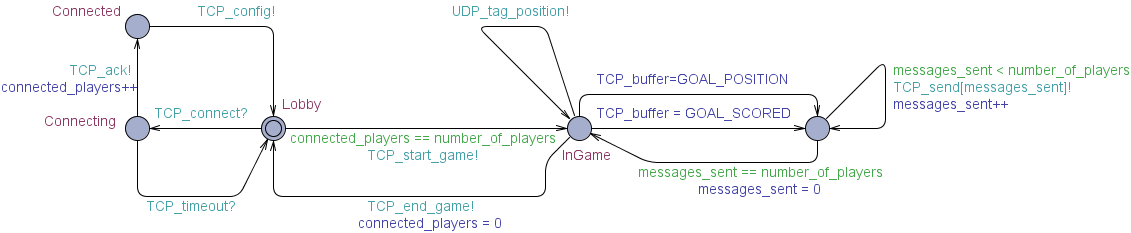
\includegraphics[width=1\linewidth]{sprint4/simplified-host.png}
    \caption{The \uppTemp{Host} template of the simplified \uppaal model.}
    \label{fig:sprint4-uppaal-simplified-host}
\end{figure}

\subsection*{Simplified Client}
The simplified client can be seen on  \autoref{fig:sprint4-uppaal-simplified-client}.
The \uppProc{Client} starts in the \uppLoc{Initial} location, it then tries to connect and transitions to \uppLoc{Connecting}.
While in \uppLoc{Connecting} it waits for an acknowledgement from the \uppProc{Host}.
If it does not receive an acknowledgement before the timeout limit it outputs a \uppOut{TCP_timeout} and transitions back to \uppLoc{Initial}.
Otherwise, if the \uppProc{Client} receives an acknowledgement from the \uppProc{Host}, it transitions to \uppLoc{Setup} and waits for the \uppProc{Host} to send configuration data.
When the \uppProc{Client} receives the configuration data it transitions to \uppLoc{Lobby} and then waits for the game to start.
When the \uppProc{Host} starts the game, all clients that are in \uppLoc{Lobby} transition to \uppLoc{InGame}.
From there, the \uppProc{Client} waits for the \uppProc{Host} to send messages.
It can receive either a TCP or UDP message, which makes it transition to \uppLoc{InGame} again, or it can receive a message that the game has ended which makes it transition to \uppLoc{Initial}.
\begin{figure}[h]
    \centering
    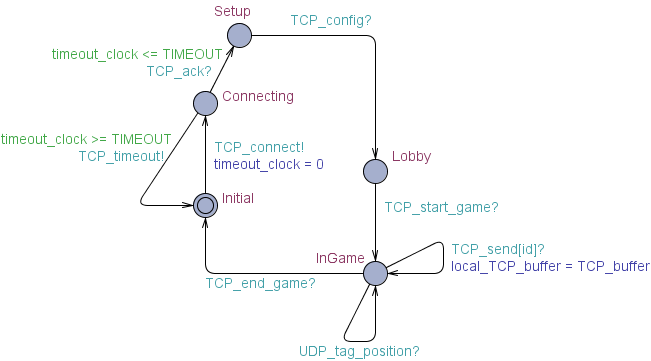
\includegraphics[width=1\linewidth]{sprint4/simplified-client.png}
    \caption{The \uppTemp{Client} template of the simplified \uppaal model.}
    \label{fig:sprint4-uppaal-simplified-client}
\end{figure}

\noindent
The more extensive \uppaal model will now be discussed and the templates in it will be described, starting with the system declarations of the model.

\subsection{System declarations}
\begin{uppaalcode}[caption={System declarations}, label={lst:uppaal4:systemdecl},captionpos=b]
    system UDP_host, TCP_host, TCP_client, Host, Client;
\end{uppaalcode}
The project consists of five templates: \uppTemp{Host}, \uppTemp{Client}, \uppTemp{TCP_client}, \uppTemp{TCP_host}, \uppTemp{UDP_host} seen in \autoref{lst:uppaal4:systemdecl}.
As mentioned above, the \uppTemp{Host} and \uppTemp{Client} templates are meant to represent the interface that users interact with when using the system.
In this new version of the model, the inclusion of \uppTemp{TCP_client}s, \uppTemp{TCP_host}s, and a \uppTemp{UDP_host} allows us to model the behavior of the network aspect of the system.

% System declarations
\subsection{Global declarations}
The global declarations (seen on \autoref{lst:uppaal4:globaldecl}) for the system have two purposes: Setting game and simulation specific options, such as how many clients should be instantiated, or how long the TCP client should wait for a response before declaring the connection as timed out.
\\
To facilitate data transfer between the templates, the model makes use of global buffers.
Each place in the \uppVar{TCP_buffer} array corresponds to a buffer related to a \uppTemp{Client} or \uppTemp{Host} process so that \uppProc(Client(0)) will read from index 0 of the array, \uppProc(Client(1)) will read from index 1 and so on.
The \uppVar{host} variable is saved as an alias to know which space in the buffers is reserved for messages from clients to the host.
Since the \uppVar{UDP_buffer} is supposed to correspond to a multicast, it is simply saved as an integer instead, which will hold the information that any client listening to the multicast will receive.
Finally, a series of channels are defined.
The channels are used to synchronize between the different processes and will be further explained when going into details about each template.

\begin{uppaalcode}[caption={Global declarations}, label={lst:uppaal4:globaldecl},captionpos=b]
const int number_of_clients = 4;
const int time_limit = 2;
const int host = number_of_clients;

typedef int[0, number_of_clients - 1] id_t;

// Each TCP instance has their own entry in the TCP buffer. The clients have the entry at index = their id and the host has the last index.
int TCP_buffer[number_of_clients + 1];
int UDP_buffer;
broadcast chan read_UDP_buffer;
chan tcp_sync[number_of_clients], ack_sync[number_of_clients], ack[number_of_clients], send_message[number_of_clients], timeout[number_of_clients];

chan TCP_send[number_of_clients], TCP_connect[number_of_clients], TCP_connected[number_of_clients], TCP_client_connected, read_TCP_buffer[number_of_clients];

chan UDP_start, UDP_send;
\end{uppaalcode}

% Host
\subsection{Host template}
The \uppTemp{Host} has three variables that are declared in \autoref{lst:sprint-4-host-code} which are:
\uppVar{connected_clients} which it uses to keep track of how many clients have connected, \uppVar{local_TCP_buffer} which is where the contents of the global TCP buffer is copied into and \uppVar{i} which it uses to keep track of how many messages it has sent.
The template seen in \autoref{fig:sprint4-uppaal-host} can be divided into three sections.
In the first section the host waits for the clients to connect through TCP.
Every time a \uppTemp{Client} has connected the \uppTemp{Host} receives a \uppIn{TCP_client_connected} synchronization and \uppVar{connected_client} is incremented.
When all of the clients have connected the \uppTemp{Host} moves on to the next section.
In this section the \uppTemp{Host} uses the \uppOut{TCP_send} synchronization to notify each \uppTemp{Client} that the game is starting through TCP.
Finally the \uppTemp{Host} is \uppLoc{InGame} and continuously sends messages to the clients.
This is done through either \uppOut{TCP_send} or \uppOut{UDP_send} which are the TCP and UDP channels respectively.
\begin{figure}[h]
    \centering
    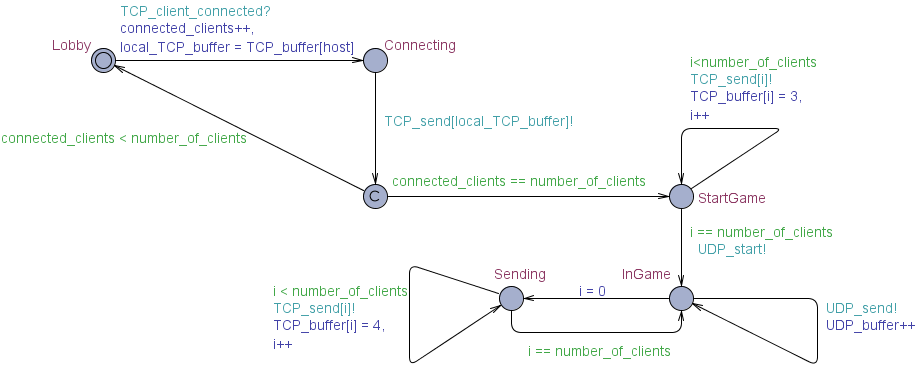
\includegraphics[width=1\linewidth]{sprint4/Host.png}
    \caption{The Host template of the \uppaal model.}
    \label{fig:sprint4-uppaal-host}
\end{figure}

\begin{uppaalcode}[caption={local Host declarations}, label={lst:sprint-4-host-code},captionpos=b]
int connected_clients = 0;
int local_TCP_buffer;
int i = 0;
\end{uppaalcode}


% Client
\subsection{Client template}
Like the \uppTemp{Host} template, the \uppTemp{Client} has a local declaration for saving the data it reads from the global buffer.
Since it is desirable to have a variable amount of instances, the template has an \uppType{id_t} parameter called \uppVar{id}, to allow instantiating multiple client processes.
The \uppTemp{Client} has four named locations, as seen on \autoref{fig:sprint4-uppaal-client}, which correspond to the states that the actual implementation can be in.
First off, the process starts in an \uppLoc{Initial} location, which then uses the \uppOut{TCP_connect[id]} to make the \uppTemp{TCP_client(id)} start connecting through TCP and transition to \uppLoc{Connecting}.
The \uppProc{Client(id)} receives \uppIn{TCP_connected[id]} synchronization when the \uppProc{TCP_client(i)} has connected and it then transitions to the \uppLoc{Lobby} location.
Everytime it receives a \uppIn{read_TCP_buffer[id]} it means that the \uppTemp{Host} sent a message.
It then transitions to an in-between location and then either transition back to \uppLoc{lobby} or to \uppLoc{InGame} depending on what message is received.
The in-between location is a committed location.
This is done so that the \uppProc{Client(id)} has to transition from it immediately instead of waiting.
Finally, there is the \uppLoc{InGame} location, which is where the client will be located most of the time during the simulation.
This indicates that the client is now in a game, and can continuously receive information about the game state through the \uppIn{read_UPD_buffer} and \uppIn{read_TCP_buffer[id]} synchronizations.
\begin{figure}[h]
    \centering
    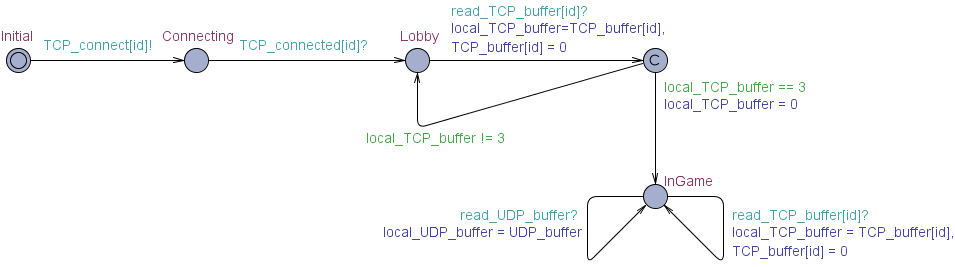
\includegraphics[width=1\linewidth]{sprint4/Client.png}
    \caption{The Client template of the \uppaal model.}
    \label{fig:sprint4-uppaal-client}
\end{figure}

% TCP
\subsection{TCP host and client templates}
The \uppTemp{TCP_Host} and \uppTemp{TCP_Client} were designed such that there will be a single process of both respectively for each client process that exists.
This was designed to model the connection that is established between the host and a client.
Like in the \uppTemp{Client}, this happens by having an \uppVar{clientId} as a parameter for when the process is instantiated.
As seen on \autoref{fig:sprint4-uppaal-tcp-client} and \autoref{fig:sprint4-uppaal-tcp-host}, the TCP templates will stay in a \uppLoc{Start} location until \uppProc{TCP_client} receive an \uppIn{TCP_connect[id]} synchronization from a \uppProc{Client}.
The \uppTemp{TCP_Host} and \uppTemp{TCP_Client} will then begin to initialize a 3-way handshake to ensure that both parties are ready for transferring data between them.
Once the handshake has been completed, the \uppTemp{TCP_Host} will send a message to the \uppTemp{Host} to inform that a new player has been connected via the \uppOut{TCP_client_connected} synchronization, and then enter an \uppLoc{Idle} location to indicate that it is ready to send messages.
Likewise, in the \uppTemp{TCP_Client}, after the handshake is completed it will inform the \uppTemp{Client} that a connection has been successfully established through the \uppOut{TCP_connected[id]} synchronization, and transition to the \uppLoc{Idle} location where it is ready to receive messages.

\begin{figure}[h]
    \centering
    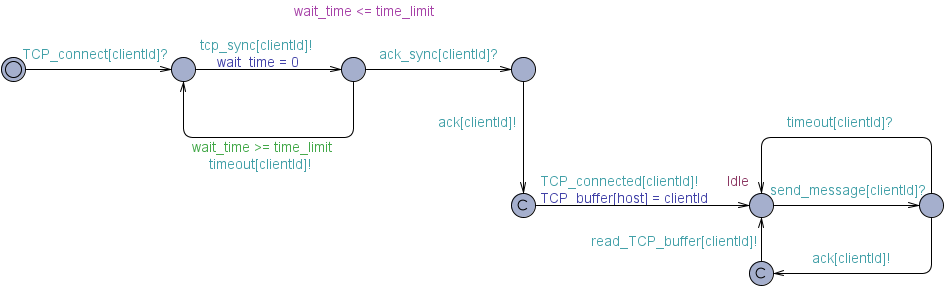
\includegraphics[width=1\linewidth]{sprint4/TCP_client.png}
    \caption{The TCP\_client template of the \uppaal model.}
    \label{fig:sprint4-uppaal-tcp-client}
\end{figure}

\begin{figure}[h]
    \centering
    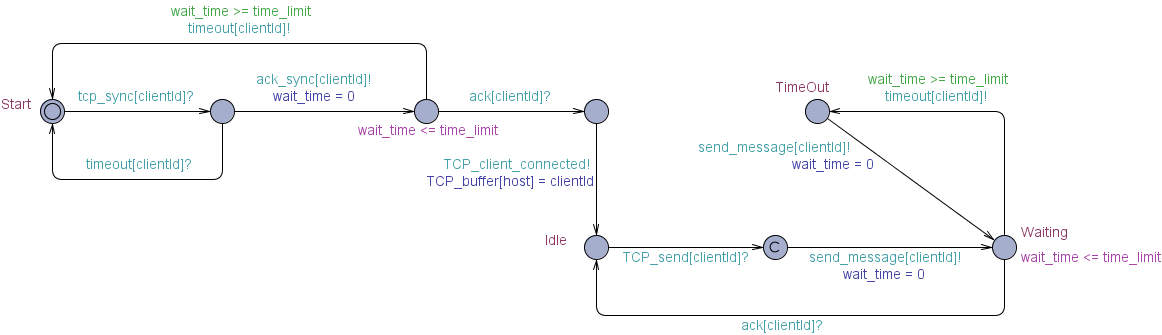
\includegraphics[width=1\linewidth]{sprint4/TCP_host.png}
    \caption{The TCP\_host template of the \uppaal model.}
    \label{fig:sprint4-uppaal-tcp-host}
\end{figure}

% UDP
\subsection{UDP host templates}
The final template seen in \autoref{fig:sprint4-uppaal-udp-host} is the \uppTemp{UDP_host}.
It is very simple as it waits until the \uppOut{Host} communicates that the games has started through \uppIn{UDP_start}.
When the \uppTemp{UDP_host} has started it waits for a \uppIn{UDP_send} synchronization from the host and then notifies the clients through the \uppOut{read_UDP_buffer} synchronization that they should read the global buffer.
\begin{figure}[h]
    \centering
    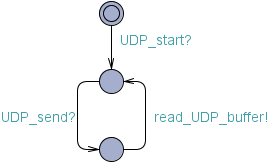
\includegraphics{sprint4/UDP_host.png}
    \caption{The UPD\_host template of the \uppaal model.}
    \label{fig:sprint4-uppaal-udp-host}
\end{figure}

% Trace example of the system
\subsection{Perfect scenario simulation trace}
In \uppaal it is possible to generate traces of simulations of the model.
This is useful when verifying different properties of the model or when getting an overview of how the model works.
A simulation trace can be seen on \autoref{fig:sprint4-happy-trace}.
At the top of the trace you see all of the processes in the system.
You can then see the trace of each process which is the line that goes from the process and to the bottom of the diagram.
The boxes on the trace indicate which Location the process is in at any given time.
The red arrows between the traces symbolize synchronizations that happen between processes, and the label on the red arrow indicates which channel it happens through.
As seen on the trace \uppTemp{Client(0)} first connects through the threeway handshake without any timeouts.
\uppTemp{Client(1)} then also connects through a three-way handshake without any timeouts.
Finally, after both of the clients are in the \uppLoc{Lobby}, the \uppTemp{Host} transitions to \uppLoc{InGame}.
\begin{figure}[H]
    \centering
    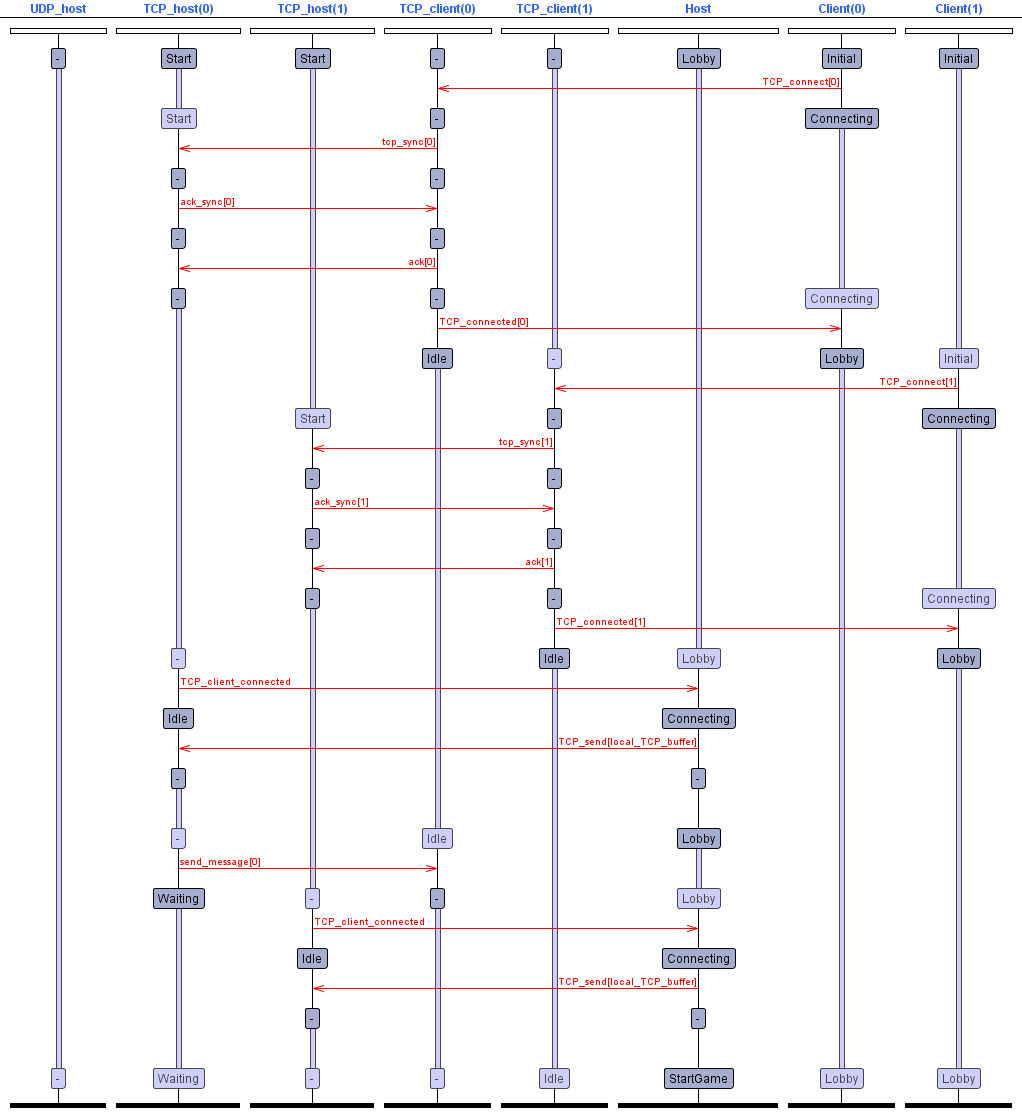
\includegraphics[width=1\linewidth]{sprint4/connected-trace.png}
    \caption{Example of a trace where both \uppProc{Client} processes connect without any problems.}
    \label{fig:sprint4-happy-trace}
\end{figure}

\subsection{Trace with a timeout}
A trace where it times out once while connecting can be seen on \autoref{fig:sprint4-timeout-trace}.
\uppTemp{Client(1)} connects without any issues, but \uppTemp{Client(0)} times out once while connecting.
This can be seen on the trace of \uppProc{TCP_client(0)}. When it sends the \uppOut{tcp_sync[0]} it times out because it does not get a response from the \uppProc{TCP_host(1)}.
It then resends the message successfully and continues with connecting.
\begin{figure}[H]
    \centering
    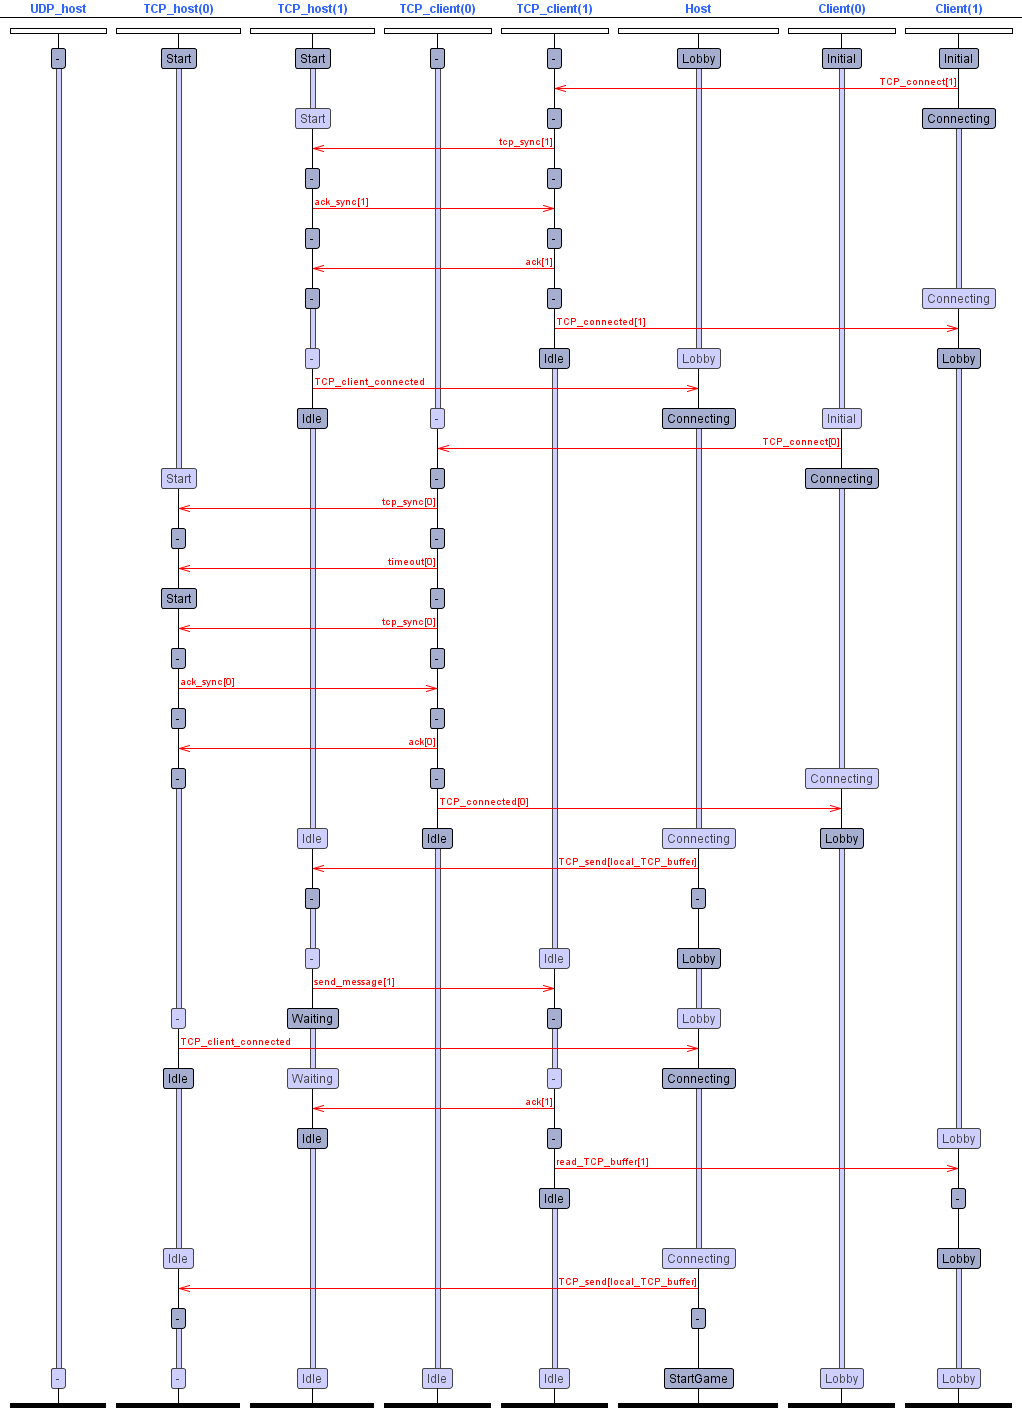
\includegraphics[width=1\linewidth]{sprint4/timeout-trace.png}
    \caption{Example of a trace where a \uppProc{TCP_host} times out while connecting.}
    \label{fig:sprint4-timeout-trace}
\end{figure}
